 \label{Chapter2}
 \setstretch{1.5}

This thesis employs some important concepts from lattice theory to address the problem of the range (or distance) estimation. In this chapter we first introduce these important concepts from lattice theory and then describe some existing techniques used in the literature for range estimation. We also describe some existing wavelengths selection methods devised for different range estimation techniques. This discussion will lay down foundations for the remainder of the thesis. This chapter is structured as follows. In Section~\ref{sec:ch2-lattice-theory} we describe some introductory concepts from lattice theory that are required for better understanding of the rest of the thesis. Some important techniques for range estimation are discussed in Section~\ref{sec:ch2-range-estimation-techniques}. Section~\ref{ch2:wavelength-selection-methods} presents wavelengths selection strategies available in the literature for different range estimation techniques.

\section{Lattice Theory}\label{sec:ch2-lattice-theory}
Historical foundations of this field were laid down by investigations of some famous mathematicians such as Gauss and Lagrange in the late 18th century and later by Minkowski. Lattices have now become a hot research topic due to its applications in wide range of problems such as cryptography and cryptanalysis, image processing, signal processing for MIMO communications, frequency estimation, and range estimation etc. In the following we provide an overview of some important concepts from lattice theory.
\begin{figure}[t]
  \centering
  \begin{tikzpicture}
%    \coordinate (Origin)   at (0,0);
%    \coordinate (XAxisMin) at (-3,0);
%    \coordinate (XAxisMax) at (5,0);
%    \coordinate (YAxisMin) at (0,-2);
%    \coordinate (YAxisMax) at (0,5);
%    \draw [thin, gray,-latex] (XAxisMin) -- (XAxisMax);% Draw x axis
%    \draw [thin, gray,-latex] (YAxisMin) -- (YAxisMax);% Draw y axis

    \clip (-3,-3) rectangle (6cm,4cm); % Clips the picture...
    \pgftransformcm{3}{0.6}{0.6}{3}{\pgfpoint{0cm}{0cm}}
          % This is actually the transformation matrix entries that
          % gives the slanted unit vectors. You might check it on
           % MATLAB etc. . I got it by guessing.
%    \coordinate (Bone) at (0,2);
%    \coordinate (Btwo) at (2,-2);
 %  \draw[style=help lines,dashed] (-14,-14) grid[step=1cm] (14,14);
          % Draws a grid in the new coordinates.
          %\filldraw[fill=gray, fill opacity=0.3, draw=black] (0,0) rectangle (2,2);
              % Puts the shaded rectangle
    \foreach \x in {-5,-4.8,...,5}{% Two indices running over each
      \foreach \y in {-5,-4.8,...,5}{% node on the grid we have drawn 
        \node[draw,circle,inner sep=1pt,fill] at (2*\x,2*\y) {};
            % Places a dot at those points
      }
    }
%    \draw [ultra thick,-latex,red] (Origin)
%        -- (Bone) node [above left] {$b_1$};
%    \draw [ultra thick,-latex,red] (Origin)
%        -- (Btwo) node [below right] {$b_2$};
%    \draw [ultra thick,-latex,red] (Origin)
%        -- ($(Bone)+(Btwo)$) node [below right] {$b_1+b_2$};
%    \draw [ultra thick,-latex,red] (Origin)
%        -- ($2*(Bone)+(Btwo)$) node [above left] {2$b_1+b_2$};
%    \filldraw[fill=gray, fill opacity=0.3, draw=black] (Origin)
%        rectangle ($2*(Bone)+(Btwo)$);
    %\draw [thin,-latex,red, fill=gray, fill opacity=0.3] (0,0)
        % -- ($2*(0,2)+(2,-2)$)
        % -- ($3*(0,2)+2*(2,-2)$) -- ($(0,2)+(2,-2)$) -- cycle;
  \end{tikzpicture}
  \caption{A lattice in $\reals^2$.}
  \label{fig:ch2-lattice-1}
\end{figure}
%00000000000000000000000000000000000000000000000000000000000000000000000

%00000000000000000000000000000000000000000000000000000000000000000000000

A \textbf{lattice} is a set of points in n-dimensional Euclidean space. It has a periodic structure as shown in Figure~\ref{fig:ch2-lattice-1}. Let $\mathbf{b}_1,....,\mathbf{b}_n$ be linearly independent vectors from $m$-dimensional Euclidean space $\reals^m$ with $m\geq n$.  The set of vectors
\[
\Lambda = \{ u_1\bbf_1 + \dots + u_n \bbf_n \mid u_1,\dots,u_n \in \ints \}
\]
is called an $n$-dimensional \term{lattice}.  The elements of $\Lambda$ are called \term{lattice points} or \term{lattice vectors}. 

The vectors $\bbf_1,\dots,\bbf_n$ form a \textbf{basis} for the lattice $\Lambda$.  We can equivalently write
\[
\Lambda=\{ \Bbf\ubf \mid \ubf \in \ints^n \}
\]
where $\Bbf$ is the $m\times n$ matrix with columns $\bbf_1,\dots,\bbf_n$. The matrix $\Bbf$ is called a \textbf{basis} or \textbf{generator} for $\Lambda$. The basis of a lattice is not unique. If $\Ubf$ is an $n \times n$ matrix with integer elements and determinant $\det\Ubf=\pm 1$ then  $\Ubf$ is called a \textbf{unimodular matrix} and $\Bbf$ and $\Bbf\Ubf$ are both bases for $\Lambda$.  When $m = n$ the lattice is said to be \textbf{full rank}. When $m > n$ the lattice points lie in the $n$-dimensional subspace of $\reals^m$ spanned by $\bbf_1,\dots,\bbf_n$.  The set of integers $\ints^n$ is called the \textbf{integer lattice} with the $n \times n$ identity matrix $\bf{I}$ as a basis.

\begin{figure}[t]
  \centering
  \begin{tikzpicture}
    \coordinate (Origin)   at (0,0);
    \coordinate (XAxisMin) at (-3,0);
    \coordinate (XAxisMax) at (5,0);
    \coordinate (YAxisMin) at (0,-2);
    \coordinate (YAxisMax) at (0,5);
    \draw [thin, gray,-latex] (XAxisMin) -- (XAxisMax);% Draw x axis
    \draw [thin, gray,-latex] (YAxisMin) -- (YAxisMax);% Draw y axis

   \clip (-3,-3) rectangle (6cm,4cm); % Clips the picture...
    \pgftransformcm{3}{0.6}{0.6}{3}{\pgfpoint{0cm}{0cm}}
          % This is actually the transformation matrix entries that
          % gives the slanted unit vectors. You might check it on
           % MATLAB etc. . I got it by guessing.
    \coordinate (Bone) at (0.0,0.4);
    \coordinate (Btwo) at (0.4,0.0);
    \coordinate (Bthree) at (-0.4,0.8);

 %  \draw[style=help lines,dashed] (-14,-14) grid[step=1cm] (14,14);
          % Draws a grid in the new coordinates.
          %\filldraw[fill=gray, fill opacity=0.3, draw=black] (0,0) rectangle (2,2);
              % Puts the shaded rectangle
    \foreach \x in {-6,-5.8,...,6}{% Two indices running over each
      \foreach \y in {-6,-5.8,...,6}{% node on the grid we have drawn  
        \node[draw,circle,inner sep=1pt,fill] at (2*\x,2*\y) {};
            % Places a dot at those points
      }
    }
    \draw [ultra thick,-latex,red] (Origin)
        -- (Bone) node [right] {$b_1$};
    \draw [ultra thick,-latex,red] (Origin)
        -- (Btwo) node [right] {$b_2$};
    \draw [ultra thick,-latex,red] (Origin)
        -- (Bthree) node [left] {$b_3$};
%    \draw [ultra thick,-latex,red] (Origin)
%        -- ($(Bone)+(Btwo)$) node [right] {$b_1+b_2$};
%    \draw [ultra thick,-latex,red] (Origin)
%        -- ($2*(Bone)+(Btwo)$) node [above right] {2$b_1+b_2$};
%    \filldraw[fill=gray, fill opacity=0.3, draw=black] (Origin)
%        rectangle ($2*(Bone)+(Btwo)$);
    %\draw [thin,-latex,red, fill=gray, fill opacity=0.3] (0,0)
        % -- ($2*(0,2)+(2,-2)$)
        % -- ($3*(0,2)+2*(2,-2)$) -- ($(0,2)+(2,-2)$) -- cycle;
  \end{tikzpicture}
  \caption{Two of the many possible basis matrices for a lattice in $\reals^2$ are shown i.e. $\Bbf_1 =[\bbf_1\quad \bbf_2]$ and $\Bbf_2 =[\bbf_1\quad \bbf_3]$.}
  \label{fig:ch2-lattice-2}
\end{figure}
%00000000000000000000000000000000000000000000000000000000000000000000000
%\textbf{Span:}
%00000000000000000000000000000000000000000000000000000000000000000000000

The \textbf{span} of a lattice $(\Lambda)$ is the linear space spanned by its vectors, that is,
\[
\text{span}(\Lambda) = \text{span}(\Bbf) = \{ \Bbf \upsilonbf | \upsilonbf \in \reals^n\}
\]
%00000000000000000000000000000000000000000000000000000000000000000000000
%\textbf{Gram matrix:}
%00000000000000000000000000000000000000000000000000000000000000000000000

Let $\Bbf$ be the basis of a lattice $\Lambda$ then the matrix
\[
\Abf = \Bbf^\prime \Bbf
\]
is called the \textbf{Gram matrix} and $\Bbf^\prime$ denotes the transpose of $\Bbf$.

%00000000000000000000000000000000000000000000000000000000000000000000000
%\textbf{Fundamental Parallelepiped:}
%00000000000000000000000000000000000000000000000000000000000000000000000

The parallelepiped formed by basis vectors $\bbf_1,\dots,\bbf_n$ is called a \textbf{fundamental parallelepiped} of the lattice $\Lambda$. For a lattice with a basis $\Bbf$ the fundamental parallelepiped $\mathcal{P}(\Bbf)$ is defined as
\[
\mathcal{P}(\Bbf) = \{\Bbf \nubf | \nubf \in \reals^n, \forall i : 0 \leq \nu_i < 1 \}
\]
A fundamental parallelepiped has $n$-dimensional volume $\sqrt{\Abf} = \sqrt{\det \Bbf^\prime\Bbf }$ where superscript $^\prime$ denotes the vector or matrix transpose.  This quantity is also called the determinant of the lattice and is denoted by $\det\Lambda$.  The fundamental parallelepiped for a two-dimensional lattice is shown in Figure~\ref{fig:ch2-parallelepiped} as the region covered by the dashed line parallelepiped. $\mathcal{P}(\Bbf)$ depends on the basis $\Bbf$. It can be observed that if we place a copy of $\mathcal{P}(\Bbf)$ at each lattice point in $\Lambda$ then we obtain tiling of the entire span$(\Lambda)$ as shown in Figure~\ref{fig:ch2-parallelepiped-tiling}.

\begin{figure}[t]
  \centering
  \begin{tikzpicture}
    \coordinate (Origin)   at (0,0);
    \coordinate (XAxisMin) at (-3,0);
    \coordinate (XAxisMax) at (5,0);
    \coordinate (YAxisMin) at (0,-2);
    \coordinate (YAxisMax) at (0,5);
%    \draw [thin, gray,-latex] (XAxisMin) -- (XAxisMax);% Draw x axis
%    \draw [thin, gray,-latex] (YAxisMin) -- (YAxisMax);% Draw y axis

   \clip (-3,-3) rectangle (6cm,4cm); % Clips the picture...
    \pgftransformcm{3}{0.6}{0.6}{3}{\pgfpoint{0cm}{0cm}}
          % This is actually the transformation matrix entries that
          % gives the slanted unit vectors. You might check it on
           % MATLAB etc. . I got it by guessing.
%    \coordinate (Bone) at (0,2);
%    \coordinate (Btwo) at (2,-2);
 % \draw[style=help lines,dashed] (-1,1) grid[step=1cm] (0,0);
  \draw[style=help lines,dashed] (0,0) -- (0,0.4);
  \draw[style=help lines,dashed] (0,0.4) -- (0.4,0.4);
  \draw[style=help lines,dashed] (0,0) -- (0.4,0);
  \draw[style=help lines,dashed] (0.4,0) -- (0.4,0.4);
          % Draws a grid in the new coordinates.
          %\filldraw[fill=gray, fill opacity=0.3, draw=black] (0,0) rectangle (2,2);
              % Puts the shaded rectangle
    \foreach \x in {-6,-5.8,...,6}{% Two indices running over each
      \foreach \y in {-6,-5.8,...,6}{% node on the grid we have drawn  
        \node[draw,circle,inner sep=1pt,fill] at (2*\x,2*\y) {};
            % Places a dot at those points
      }
    }
%    \draw [ultra thick,-latex,red] (Origin)
%        -- (Bone) node [above left] {$b_1$};
%    \draw [ultra thick,-latex,red] (Origin)
%        -- (Btwo) node [below right] {$b_2$};
%    \draw [ultra thick,-latex,red] (Origin)
%        -- ($(Bone)+(Btwo)$) node [below right] {$b_1+b_2$};
%    \draw [ultra thick,-latex,red] (Origin)
%        -- ($2*(Bone)+(Btwo)$) node [above left] {2$b_1+b_2$};
%    \filldraw[fill=gray, fill opacity=0.3, draw=black] (Origin)
%        rectangle ($2*(Bone)+(Btwo)$);
    %\draw [thin,-latex,red, fill=gray, fill opacity=0.3] (0,0)
        % -- ($2*(0,2)+(2,-2)$)
        % -- ($3*(0,2)+2*(2,-2)$) -- ($(0,2)+(2,-2)$) -- cycle;
  \end{tikzpicture}
  \caption{Fundamental parallelepiped formed by the basis $\Bbf_1 =[\bbf_1\quad \bbf_2]$.}
  \label{fig:ch2-parallelepiped}
\end{figure}

\begin{figure}[t]
  \centering
  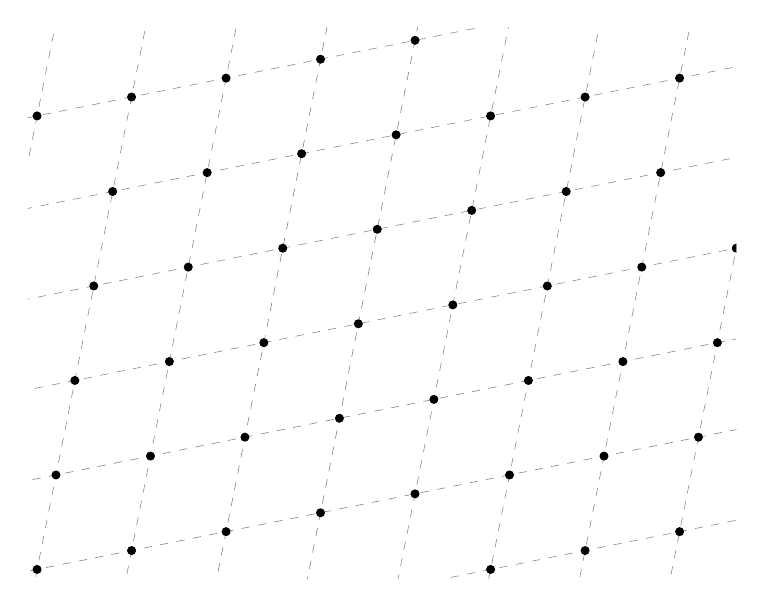
\begin{tikzpicture}
    \coordinate (Origin)   at (0,0);
    \coordinate (XAxisMin) at (-3,0);
    \coordinate (XAxisMax) at (5,0);
    \coordinate (YAxisMin) at (0,-2);
    \coordinate (YAxisMax) at (0,5);
%    \draw [thin, gray,-latex] (XAxisMin) -- (XAxisMax);% Draw x axis
%    \draw [thin, gray,-latex] (YAxisMin) -- (YAxisMax);% Draw y axis

    \clip (-3,-3) rectangle (6cm,4cm); % Clips the picture...
    \pgftransformcm{3}{0.6}{0.6}{3}{\pgfpoint{0cm}{0cm}}
          % This is actually the transformation matrix entries that
          % gives the slanted unit vectors. You might check it on
           % MATLAB etc. . I got it by guessing.
%    \coordinate (Bone) at (0,2);
%    \coordinate (Btwo) at (2,-2);
 \draw[style=help lines,dashed] (-6,-6) grid[step=0.4cm] (6,6);
          % Draws a grid in the new coordinates.
          %\filldraw[fill=gray, fill opacity=0.3, draw=black] (0,0) rectangle (2,2);
              % Puts the shaded rectangle
    \foreach \x in {-6,-5.8,...,6}{% Two indices running over each
      \foreach \y in {-6,-5.8,...,6}{% node on the grid we have drawn  
        \node[draw,circle,inner sep=1pt,fill] at (2*\x,2*\y) {};
            % Places a dot at those points
      }
    }
%    \draw [ultra thick,-latex,red] (Origin)
%        -- (Bone) node [above left] {$b_1$};
%    \draw [ultra thick,-latex,red] (Origin)
%        -- (Btwo) node [below right] {$b_2$};
%    \draw [ultra thick,-latex,red] (Origin)
%        -- ($(Bone)+(Btwo)$) node [below right] {$b_1+b_2$};
%    \draw [ultra thick,-latex,red] (Origin)
%        -- ($2*(Bone)+(Btwo)$) node [above left] {2$b_1+b_2$};
%    \filldraw[fill=gray, fill opacity=0.3, draw=black] (Origin)
%        rectangle ($2*(Bone)+(Btwo)$);
    %\draw [thin,-latex,red, fill=gray, fill opacity=0.3] (0,0)
        % -- ($2*(0,2)+(2,-2)$)
        % -- ($3*(0,2)+2*(2,-2)$) -- ($(0,2)+(2,-2)$) -- cycle;
  \end{tikzpicture}
  \caption{Tiling of the entire $span(\Lambda)$ by parallelepiped placed at each lattice point.}
  \label{fig:ch2-parallelepiped-tiling}
\end{figure}

%\textbf{Voronoi Cell:}

The (closed) \textbf{Voronoi cell}, denoted $\vor\Lambda$, of an $n$-dimensional lattice $\Lambda$ in $\reals^m$ is the subset of $\reals^m$ containing all points nearer or of equal distance (here with respect to the Euclidean norm) to the lattice point at the origin than to any other lattice point. If the lattice is full rank so that $n=m$ then the volume of the Voronoi cell is equal to the volume of a fundamental parallelepiped, that is, $\det\Lambda$.  Otherwise, if the $m > n$ the Voronoi cell is unbounded in those directions orthogonal to the subspace spanned by the basis vectors $\bbf_1,\dots,\bbf_n$.  Specifically, if $\xbf$ is contained in this orthogonal subspace, then $\ybf \in \vor\Lambda$ if and only if $\ybf + s \xbf \in \vor\Lambda$ for all $s \in \reals$.   In this case, the intersection of the Voronoi cell with the subspace spanned by $\bbf_1,\dots,\bbf_n$ has $n$-dimensional volume equal to $\det\Lambda$.  

The Voronoi cell $\vor\Lambda$ tessellates $\reals^N$ in the sense that
\[
\reals^N = \bigcup_{\xbf \in \Lambda} (\vor\Lambda + \tbf)
\]
and $\vor\Lambda$ and a translate $\vor\Lambda + \tbf$ by a lattice point $\tbf \in \Lambda\backslash  \{\zerobf\}$ intersect at most on the boundary of $\vor\Lambda$.  The set $\Lambda \backslash  \{\zerobf\}$ denotes those lattice points from $\Lambda$ not equal to the origin $\zerobf$.  In particular, if $\interior\Lambda$ denotes the interior of the Voronoi cell, then the intersection of $\interior\Lambda$ and $\vor \Lambda + \tbf$ is empty for all $\tbf \in \Lambda \backslash  \{\zerobf\}$.  % Equivalently, if $\tbf \in \Lambda$, $\wbf \in \vor\Lambda$, and $\ybf \int\Lambda$, and
% \[
% \]
This leads to the following simple property that we will find useful.

\begin{remark}\label{remarksimpleintvor}
If $\sbf \in \Lambda$, $\tbf \in \vor\Lambda$, $\ubf \in \interior\Lambda$, and $\tbf = \ubf + \sbf$, then $\sbf = \zerobf$.
\end{remark}

%\textbf{Hyperballs:}

Let $R$ denote the radius of an n-dimensional \textbf{Euclidean ball}. The volume $V_n$ of this ball is given as
\[
V_n = \frac{\pi^{n/2}R^n}{\Gamma(n/2 + 1)} 
\]
where $\Gamma$ is the Gamma function $\Gamma(n)=(n-1)!$ for $n\in \ints^+$. The radius of this ball can be expressed as
\[
R =  \dfrac{\left (V_n \Gamma(n/2 + 1)\right)^{1/n}}{\sqrt{\pi}} 
\]

The probability $P_r(\Lambda, \sigma^2)$ that an independent and identically distributed n-variate Gaussian random variable lies inside the Voronoi cell can be upper bounded by the probability that this n-variate Gaussian random variable lies within a ball of volume equal to that of the Voronoi cell~\cite[Sec.~IV.C]{Hassibi_GPS_1998}, i.e.,
\begin{equation}\label{ch2:upperBoundUsingSphere}
P_r(\Lambda, \sigma^2) \leq F_n \left( \frac{ \left (  \Gamma(n/2 + 1)  \text{det}\Lambda  \right)^{2/n} } {\pi \sigma^2} \right)
\end{equation}
where $F_n(x)$ is the chi-square cumulative distribution function with $n$ degrees of freedom,  $\Gamma(x)$ is the gamma function.

A \textbf{short vector} in a lattice $\Lambda$ is a lattice point of minimum nonzero Euclidean length, that is, a lattice point of length
\[
\dmin =  \min_{\xbf \in \Lambda \backslash \{ \zerobf \} } \| \xbf \|^2.
\]   
The length $\dmin$ of a short vector is the smallest distance between any two lattice points. 

The \textbf{inradius} or \textbf{packing radius} $\rho = \dmin/2$ is the length of a point on the boundary of the Voronoi cell that is closest to the origin (Figure~\ref{fig:bound_dmin}).  Equivalently, the inradius is the radius of the largest sphere that fits inside the Voronoi cell.  It is also the radius of the largest sphere that can be centered at each lattice point such that no two spheres intersect.  Such an arrangement of spheres is called a \textbf{sphere packing} (Figure~\ref{fig:bound_dmin}).

\begin{figure}[t]
\begin{center}   
\includegraphics{chapters/ch2/figs/latticefigures-1.mps}
\caption{The inradius $\rho = \dmin/2$ of the 2-dimensional lattice with basis $\bbf_1 = [3,0.72]^\prime, \bbf_2 = [0.6,3.6]^\prime$. The dots are the lattice points.  The origin $\zerobf$ is the lattice point in the center of the figure.  This lattice has two short vectors.  The shaded region shows the Voronoi cell of the lattice.  The solid circles exhibit a sphere packing.  The dashed circle has area (2-volume) equal to that of the Voronoi cell. The sphere with volume equal to the Voronoi cell is used in the upper bound~\ref{upperBoundUsingSphere}.}
\label{fig:bound_dmin}
\end{center}  
\end{figure} 

%\textbf{Dual Lattice}

Let $\Lambda$ be an $n$-dimensional lattice and let $H$ be the $n$-dimensional subspace spanned by its lattice points. The \textbf{dual lattice} of $\Lambda$, denoted $\Lambda^*$, contains those points from $H$ that have integer inner product with all points from $\Lambda$, that is,
\[
\Lambda^* = \{ \xbf  \in H \mid \xbf^\prime \bar{\xbf} \in \ints \text{ for all } \bar{\xbf} \in \Lambda \}.
\]
The determinant of a lattice and its dual are reciprocals, that is, $\det\Lambda = (\det\Lambda^*)^{-1}$~\cite[p. 10]{SPLAG}.  A lattice and its dual have interesting properties when intersected with or projected onto a subspace.  %These properties will be particularly useful for the purpose of range estimation.

\begin{proposition} \label{prop:ch2-projectedintersection}
Let $\Lambda\subset\reals^n$ be an $n$ dimensional lattice, and let $H$ be a $n-k$ dimensional subspace of $\reals^n$.  Let $H^\perp$ be the $k$ dimensional space orthogonal to $H$ and let $p$ be the orthogonal projection onto $H$.  The set $\Lambda \cap H$ is an $n-k$ dimensional lattice if and only if $\Lambda \cap H^\perp$ is a $k$ dimensional lattice.  Moreover, if $\Lambda \cap H$ is an $n-k$ dimensional lattice then:
\begin{enumerate}
\item The dual of $\Lambda \cap H$ is the orthogonal projection of $\Lambda^*$ onto $H$, that is, $(\Lambda \cap H)^* = p(\Lambda^*)$.
\item The determinants of $\Lambda$, $\Lambda \cap H$ and $\Lambda^* \cap H^{\perp}$ are related by $\det(\Lambda) \det(\Lambda^* \cap H^{\perp}) = \operatorname{det}(\Lambda \cap H)$.
\end{enumerate}
\end{proposition}
\begin{proof}
Proposition~1.3.4 and Corollary~1.3.5 of \cite{Martinet2003}.
\end{proof}

For the purpose of range estimation we will be particularly interested in Proposition~\ref{prop:ch2-projectedintersection} when $\Lambda$ is the integer lattice $\ints^n$ and $k = 1$.  We state this special case in the following corollary.

\begin{corollary} \label{cor:intlatticedim1}
Let $\vbf\in\ints^n$, let $H$ be the $n-1$ dimensional subspace orthogonal to $\vbf$, and let
\[
\Qbf = \Ibf - \frac{\vbf\vbf^\prime}{\vbf^\prime\vbf} = \Ibf - \frac{\vbf\vbf^\prime}{\|\vbf\|^2}
\]
be the $n\times n$ orthogonal projection matrix onto $H$.  The set of vectors $\ints^n\cap H$ is an $n-1$ dimensional lattice with determinant 
\[
\det(\ints^n \cap H) = \|\vbf\|
\]
and dual lattice
\[
(\ints^n \cap H)^* = \{ \Qbf \zbf \mid \zbf \in \ints^n \}.
\]
\end{corollary}

%Given a lattice $\Lambda$ in $\reals^m$ and a vector $\ybf \in \reals^m$, a problem of interest is to find a lattice point $\xbf \in \Lambda$ such that the squared Euclidean norm
%\[
%\| \ybf - \xbf \|^2 = \sum_{i=1}^m (y_i - x_i)^2
%\] 
%is minimised.  This is called the \term{closest lattice point problem} (or \term{closest vector problem}) and a solution is called a \term{closest lattice point} (or simply \term{closest point}) to $\ybf$ \cite{Agrell2002, MicciancioVoulgaris_deterministic_jv_2013}.  The closest lattice point problem and the Voronoi cell are related in that $\xbf\in\Lambda$ is a closest lattice point to $\ybf$ if and only if $\ybf - \xbf \in \vor\Lambda$. 
% A related problem is to find a lattice point of minimum nonzero Euclidean length, that is, a lattice point of length
% \[
% \min_{\xbf\in \Lambda \backslash \{ \zerobf \} } \| x \|^2,
% \]
% where $\Lambda \backslash  \{\zerobf\}$ denotes the set of lattice points not equal to the origin $\zerobf$.  This is called the \emph{shortest vector problem}.  

% The closest lattice point problem and the shortest vector problem have interested mathematicians and computer scientists due to their relationship with integer programming~\cite{Lenstra_integerprogramming1983,Kannan1987_fast_general_np,Babai1986}, the factoring of polynomials~\cite{Lenstra1982}, and 
%cryptanalysis~\cite{Joux_toolbox_cryptanal1998,NyguyenStern_two_faces_crypto,Micciancio_lattice_based_post_quantum_crypto}.  

%\textbf{Closest lattice point problem}

Given a vector $\bbf \in \reals^m$, a problem of interest is to find a lattice point $\xbf \in \Lambda$ such that the squared Euclidean norm
\[
\| \bbf - \xbf \|^2 = \sum_{i=1}^m (b_i - x_i)^2 
\]  
is minimised.  This is called the \textbf{closest lattice point problem} (or \textbf{closest vector problem}) and a solution is called a \textbf{closest lattice point} (or simply \textbf{closest point}) to $\bbf$ \cite{Agrell2002,McKilliam2009CoxeterLattices,MicciancioVoulgaris_deterministic_jv_2013,McKilliam_closest_point_lattice_first_kind_2014}.  The closest lattice point problem and the Voronoi cell are related in that $\xbf\in\Lambda$ is a closest point to $\bbf$ if and only if $\bbf - \xbf \in \vor\Lambda$.  

%\textbf{Short vector}
%The closest lattice point problem has numerous engineering applications. For example, the closest lattice point corresponds to the minimum distortion point when a lattice is used as a quantiser and it is called lattice decoding when a lattice is used to construct codes~\cite{Conway1983VoronoiCodes,Erex2004_lattice_decoding}. The problem also occurs in communications systems involving multiple antennas~\cite{Wubben_2011} and has also found applications to circular statistics~\cite{McKilliam_mean_dir_est_sq_arc_length2010}, single frequency estimation~\cite{McKilliamFrequencyEstimationByPhaseUnwrapping2009}, and related signal processing problems~\cite{Clarkson2007,McKilliam2009IndentifiabliltyAliasingPolyphase,McKilliam_pps_unwrapping_tsp_2014,McKilliam_fast_sparse_period_est_2015}. In the context of range estimation from phase observations, the closest lattice point problem has been applied by Teunissen~\cite{Teunissen_GPS_1995}, Hassibi and Boyd~\cite{Hassibi_GPS_1998} and more recently Li~et.~al.~\cite{Li_distance_est_wrapped_phase, Li_coloured_range_est_case}.
%
%The closest lattice point problem is known to be NP-hard under certain conditions when the lattice itself, or rather a basis thereof, is considered as an additional input parameter~\cite{micciancio_hardness_2001, Dinur2003_approximating_CVP_NP_hard, Jalden2005_sphere_decoding_complexity}. Nevertheless, algorithms exist that can compute a closest lattice point in reasonable time if the dimension is small (less that about 60)~\cite{Agrell2002,MicciancioVoulgaris_deterministic_jv_2013}.  %Since the paper of Viterbo and Boutros~\cite{Viterbo_sphere_decoder_1999}, these algorithms have gone by the name ``sphere decoders'' in the communications engineering and signal processing literature. 
%	Although the problem is NP-hard in general, fast algorithms are known for specific highly regular lattices~\cite{Conway1982FastQuantDec, Conway1986SoftDecLeechGolay,McKilliam2009CoxeterLattices, McKilliam_closest_point_lattice_first_kind_2014}.  For the purpose of range estimation the dimension of the lattice will be $N-1$ where $N$ is the number of frequencies transmitted.  Usually $N$ is not large.  In this case general purpose algorithms for computing a closest lattice point, such as those described in~\cite{Agrell2002}, are fast.  
	
The closest lattice point problem has numerous engineering applications.  For example, if a lattice is used as a vector quantiser then the closest lattice point corresponds to the minimum distortion point~\cite{Conway1983VoronoiCodes,Conway1982VoronoiRegions,Conway1982FastQuantDec}.  If the lattice is used as a code, then the closest lattice point corresponds to what is called \term{lattice decoding}\index{lattice decoding} and has been shown to yield arbitrarily good codes~\cite{Erex2004_lattice_decoding,Erez2005}.  The problem also occurs in communications systems involving multiple antennas~\cite{Ryan2008,Wubben_2011} and has found applications to circular statistics~\cite{McKilliam_mean_dir_est_sq_arc_length2010}, single frequency estimation~\cite{McKilliamFrequencyEstimationByPhaseUnwrapping2009}, and related signal processing problems~\cite{McKilliam2007,Clarkson2007,McKilliam2009IndentifiabliltyAliasingPolyphase,Quinn_sparse_noisy_SSP_2012}.  In the context of range estimation from phase observations, the closest lattice point problem has previously been applied by numerous authors including Teunissen~\cite{Teunissen_GPS_1995}, Hassibi and Boyd~\cite{Hassibi_GPS_1998} and more recently Li~et.~al.~\cite{Li_distance_est_wrapped_phase}.

The closest lattice point problem is known to be NP-hard under certain conditions when the lattice itself, or rather a basis thereof, is considered as an additional input parameter~\cite{micciancio_hardness_2001, Dinur2003_approximating_CVP_NP_hard, Jalden2005_sphere_decoding_complexity}. Nevertheless, algorithms exist that can compute a closest lattice point in reasonable time if the dimension is small (less that about 60)~\cite{Pohst_sphere_decoder_1981,Kannan1987_fast_general_np,Agrell2002,Viterbo_sphere_decoder_1999,Micciancio09adeterministic,schnorr_euchner_sd_1994}.  Since the paper of Viterbo and Boutros~\cite{Viterbo_sphere_decoder_1999}, these algorithms have gone by the name ``sphere decoders'' in the communications engineering and signal processing literature. 

Although the problem is NP-hard in general, fast algorithms are known for specific highly regular lattices~\cite{Conway1982FastQuantDec, Conway1986SoftDecLeechGolay,McKilliam2009CoxeterLattices, McKilliam_closest_point_lattice_first_kind_2014}.  For the purpose of range estimation the dimension of the lattice will be $N-1$ where $N$ is the number of frequencies transmitted.  Usually $N$ is not large.  In this case general purpose algorithms for computing a closest lattice point, such as those described in~\cite{Agrell2002}, are fast. 
%00000000000000000000000000000000000000000000000000000000000000000000000



%Let $\Lambda$ be an $n$-dimensional lattice and let $H$ be the $n$-dimensional subspace spanned by its lattice points. The \term{dual lattice} of $\Lambda$, denoted $\Lambda^*$, contains those points from $H$ that have integer inner product with all points from $\Lambda$, that is,
%\[
%\Lambda^* = \{ \xbf  \in H \mid \xbf^\prime \ybf \in \ints \text{ for all } \ybf \in \Lambda \}.
%\] 
% 


% For a given lattice $\Lambda$ with generator matrix $\mathbf{B}$, the minimum distance of the lattice or the length shortest lattice vector $d_{\min}$ is defined as 
  
%  \[
%  d_{\min} = \underset{\zbf \in \mathbf{\ints}^n , \zbf\neq 0}{\operatorname{min}} \|\mathbf{Bz} \|. 
%  \]
%  $d_{\min}$ is the length of the shortest lattice vector other than origin i.e. it is the distance between the origin and its closest lattice point as shown in Figure~\ref{fig:bound_dmin}. The inradius of a lattice is equal to the half of the length of the shortest lattice vector i.e. $\frac{d_{\min}}{2}$.
 


%**********************************************************************************************************************************************************************************
%\section{Range Estimation and Phase Ambiguity Problem}\label{sec:ch2-range-estimation}
%*********************************************************************************************************************************************************************************
%Range (or distance) estimation is an important component of modern technologies such as electronic surveying~\cite{Jacobs_ambiguity_resolution_interferometery_1981, anderson1998surveying} and global positioning systems (GPS)~\cite{Teunissen_GPS_LAMBDA_2006,Teunissen_GPS_1995}.  Common methods of range estimation are based upon received signal strength~\cite{Chitte_RSS_Estimation2009, HingCheung_RSSbasedRangeEstimation2012}, time of flight (or time of arrival)~\cite{XinrongLi_TOA_range_estimation2004, Lanzisera_TOA_range_estimation2011}, and phase of arrival~\cite{Jacobs_ambiguity_resolution_interferometery_1981,Towers_frequency_selection_interferometry_2003,Li_distance_est_wrapped_phase}.  This thesis focuses on the phase of arrival method which provides the most accurate range estimates in many applications.  Phase of arrival has become the technique of choice in modern high precision surveying and global positioning ~\cite{Odijk-nteger-ambiguity-resolutionPPP, Teunissen_GPS_LAMBDA_2006, Teunissen_GPS_1995}. A difficulty with phase of arrival is that only the principal component of the phase can be observed, that is, the observed value of the phase lies within the interval $[-\pi, \pi)$.  This limits the range that can be unambiguously estimated.  One approach to address this problem is to utilise signals of multiple different wavelengths and observe the phase at each. The range can then be measured within an interval of length equal to the least common multiple of these wavelengths. 
%
%Range estimators from such observations have been studied by numerous authors~\cite{Teunissen_GPS_1995,Hassibi_GPS_1998,Towers_frequency_selection_interferometry_2003,Towers:04_generalised_frequency_selection,Li_distance_est_wrapped_phase, Xia2007, XWLi2008,Xiao_multistage_crt_2014}.  Techniques include the beat wavelength method of Towers~et.~al.~\cite{Towers_frequency_selection_interferometry_2003,Towers:04_generalised_frequency_selection}, the method of excess fractions~\cite{Falaggis_excess_fractions_2013}, and methods based on the Chinese Remainder Theorem (CRT)~\cite{Oystein_Ore_general_chinese_Remainder_1952,Yuke_new_CRT_1998, Oded_Chinese_remaindering_with_errors_2000, G.Wang_location_and_imaging_2004, Xia_generalised_CRT_2005, Xia2007, XWLi2008, Xiaowei_Li_robust_CRT_2009, W.Wang_closed_form_crt_2010, Xiaowei_Li_location_and_imaging_2011, YangBin_range_estimation_with_CRT_2014, Xiao_multistage_crt_2014}.  Least squares/maximum likelihood and maximum a posteriori (MAP) estimators of range have been studied by Teunissen~\cite{Teunissen_GPS_1995}, Hassibi and Boyd~\cite{Hassibi_GPS_1998}, and more recently by Li~et.~al.~\cite{Li_distance_est_wrapped_phase}.  A key realisation is that least squares and MAP estimators can be computed by solving a problem from computational number theory known as the~\emph{closest lattice point problem}~\cite{Babai1986,Agrell2002}.  Teunissen~\cite{Teunissen_GPS_1995} appears to have been the first to have realised this connection. 
%
%Common range estimators are based upon received signal strength~\cite{Chitte_RSS_Estimation2009, HingCheung_RSSbasedRangeEstimation2012}, time of flight (or time of arrival)~\cite{XinrongLi_TOA_range_estimation2004, Lanzisera_TOA_range_estimation2011}, and phase of arrival~\cite{Jacobs_ambiguity_resolution_interferometery_1981,Towers_frequency_selection_interferometry_2003,Li_distance_est_wrapped_phase}.  %This thesis focuses on the least squares estimation of range based on the phase of arrival method that will be discussed in Chapter~\ref{Chapter3}. 
%In this section we describe some important range estimation methods from multiple phase measurements. A good understanding of these methods will be helpful for comparison with the least squares range estimator in the later chapters.

%**********************************************************************************************************************************************************************************
\section{Range Estimation Techniques}\label{sec:ch2-range-estimation-techniques}
%*********************************************************************************************************************************************************************************
%Common range estimators are based upon received signal strength~\cite{Chitte_RSS_Estimation2009, HingCheung_RSSbasedRangeEstimation2012}, time of flight (or time of arrival)~\cite{XinrongLi_TOA_range_estimation2004, Lanzisera_TOA_range_estimation2011}, and phase of arrival~\cite{Jacobs_ambiguity_resolution_interferometery_1981,Towers_frequency_selection_interferometry_2003,Li_distance_est_wrapped_phase}. This thesis focuses on the least squares estimation of range based on the phase of arrival method that will be discussed in Chapter~\ref{Chapter3}. 
In this section we describe some important range estimators that employ multiple phase observations to estimate the unknown range.  A good understanding of these methods will be helpful for comparison with the least squares range estimator in later chapters. These range estimators are based upon: (i) the beat wavelength method, (ii) the method of excess fractions, and (iii) the CRT based method. %We first briefly describe the notation used in this work. 
%Suppose that a multi-wavelength interferometer (MWI) with $N$  measurement wavelengths $\lambda_1, \ldots, \lambda_N$ is used to measure an unknown distance $r_0$. Let $\varphi_1,\ldots,\varphi_N$ be the corresponding estimated values of the interferometer phases. These phase values lie in the interval $[-\pi, \pi]$. The estimated interferometer phase $\varphi_n$ corresponding to the wavelengths $\lambda_n$ can also be related to a so called \emph{fractional fringe value} $e_n$ defined as
%\[
%\eta_n = \varphi_n/2\pi
%\]
%Suppose that a transmitter sends a signal of the form
%\begin{equation}\label{eq:xtranssignal}
%x(t) = \sin (2\pi ft + 2\pi\phi)
%\end{equation}
%of known phase $\phi$ and frequency $f$ in Hertz.  The signal is assumed to propogate by line of sight to a reciever resulting in the signal 
%\begin{equation}
%y(t) = \alpha x(t - r_0/c) + w(t) = \alpha \sin (2\pi ft + 2\pi\varphi) + w(t)
%\end{equation}
%where $r_0$ is the distance (or range) in meters between receiver and transmitter, $c$ is the speed at which the signal propagates in meters per second, $\alpha$ is the amplitude of the received signal, $w(t)$ represents noise,
%\begin{equation}
%\varphi = \phi - \dfrac{ f }{c}r_0 = \phi - \dfrac{r_0}{\lambda}
%\end{equation}
%is the phase of the received signal, and $\lambda = c/f$ is the wavelength.  Alternatively, the transmitter and receiver could be in the same location and the receiver obtains the signal after being reflected off a target.  In this case the range of the target would be $r_0/2$.
%
%Our aim is to estimate $r_0$ from the signal $y(t)$.  To do this we first calculate an estimate $\hat{\varphi}$ of the principal component of the phase $\varphi$.  In optical ranging applications $\hat{\varphi}$ might be given by an interferometer.  In sonar or radio frequency ranging applications $\hat{\varphi}$ might be obtained from the complex argument of the demodulated signal $y(t)e^{-2\pi j f t}$.  Whatever the method of phase estimation, 
%The range $r_0$ is related to the phase estimates $\hat{\varphi}_n$ by the phase differences
%\begin{equation}
%Y = \sfracpart{\phi - \hat{\varphi}} = \sfracpart{ r_0/\lambda + \Phi }
%\end{equation}
%where $\Phi$ represents phase noise and $\sfracpart{x} = x - \floor{x + \tfrac{1}{2}}$ where $\floor{x}$ denotes the greatest integer less than or equal to $x$.  %That is, $\fracpart{x}$ is the \emph{centered} fractional part of $x$. %For the purpose of analysis, it is convenient to model the phase noise using the~\emph{wrapped normal distribution}~\cite[p.~50]{Mardia_directional_statistics}\cite[p.~76]{McKilliam2010thesis}\cite[p.~47]{Fisher1993}.  That is, we model the phase noise as $\fracpart{\Phi}$ where $\Phi$ is normally distributed with zero mean. With this assumption $\hat{\varphi} = \fracpart{ \varphi - \fracpart{\Phi} } = \fracpart{ \varphi - \Phi } $ and so, the phase noise may equivalently be modelled as normally distributed \emph{without wrapping} ~\cite{Hassibi98,WenchaoLi2013}.
%For all integers $k$, 
%\begin{equation}
%Y = \fracpart{ r_0/\lambda + \Phi } = \sfracpart{(r_0 + k\lambda)/\lambda + \Phi}
%\end{equation}
%and so the range is identifiable only if $r_0$ is assumed to lie in an interval of length $\lambda$.  A natural choice is the interval $[0, \lambda)$. This poses a problem if the range $r_0$ is larger than the wavelength $\lambda$.  To alleviate this, a common approach is to transmit multiple signals %$x_1(t),\ldots,x_N(t)$
%$x_n(t) = \sin (2\pi f_nt + 2\pi\phi)$ for $n = 1,\dots,N$, each with a different frequency $f_n$.  Now $N$ phase estimates $\hat{\varphi}_1,\dots,\hat{\varphi}_N$ are computed along with phase differences 
%\begin{equation}\label{eq:Yndefn}
%Y_n = \sfracpart{\phi - \hat{\varphi}_n} = \fracpart{ r_0/\lambda_n + \Phi_n} \qquad n = 1,\dots,N
%\end{equation}
%where $\lambda_n = c/f_n$ is the wavelength of the $n$th signal and $\Phi_1,\dots,\Phi_N$ represent phase noise. 
%The relationship between the so called \emph{wrapping variables} (or integer fringe orders) $z_n$ that are related to the whole number of wavelengths that occur over the range, the fractional fringe order $\eta_n$ and the unknown range $r_0$ is given by
%\begin{equation}\label{eq:r0-zn-yn}
%r_0 = (z_n + \eta_n)\lambda_n \quad n=1,\ldots,N
%\end{equation}
In the following subsections we briefly describe these range estimators. 
\subsection{Beat Wavelength Method}
First we describe the notation used for the beat wavelength method and the method of excess fractions. Suppose that a multi-wavelength interferometer (MWI) with $N$  measurement wavelengths $\lambda_1< \lambda_2< \cdots< \lambda_N$ is used to measure an unknown distance $r_0$. Let $\varphi_1,\ldots,\varphi_N$ be the corresponding estimated values of the interferometer phases. These phase values lie in the interval $[-\pi, \pi]$. The estimated interferometer phase $\varphi_n$ corresponding to the wavelengths $\lambda_n$ can also be related to a so called \emph{fractional fringe value} $e_n$ defined as~\cite{Falaggis-generalized-th-of-PU-2012}
\[
e_n = \varphi_n/2\pi.
\]
where $e_n$ is wrapped into the interval $[-0.5, 0.5]$. The relationship between the so called \emph{wrapping variables} (or integer fringe orders) $z_n$ that are related to the whole number of wavelengths that occur over the range, the fractional fringe order $e_n$ and the unknown range $r_0$ is given by
\begin{equation}\label{eq:r0-zn-yn}
r_0 = (z_n + e_n)\lambda_n, \qquad n=1,\ldots,N
\end{equation}

The beat wavelength method, introduced by Wyant~\cite{Wyant:71}, provides direct calculation of the wrapping variables. The maximum measurable distance using the beat wavelength approach is equal to the largest beat wavelength. 
%In the following we describe the two wavelength and multi-wavelength interferometry using the beat wavelength method.
%\subsubsection{Two Wavelength Interferometry}
%In two wavelength interferometry two measurement wavelengths $\lambda_1$ and $\lambda_2$ are used to measure the unknown range.  Let $\varphi_1$ and $\varphi_2$ be the wrapped phases and $z_1$ and $z_2$ be the wrapping variables (or integer fringe orders) at wavelengths $\lambda_1$ and $\lambda_2$. In beat wavelength method, the beat wavelength and the beat phase are defined respectively as
%\[
%\Lambda_{12} = \dfrac{\lambda_1\lambda_2}{(\lambda_2 - \lambda_1)}
%\]
%and
%\[
%\Theta_{12} = \varphi_2 - \varphi_1,
%\]
%which is normally wrapped into the interval $[-\pi, \pi)$ and the fringe order (wrapping variable) is 
%\[
%Z_{12} = z_1 - z_2.
%\] 
%The maximum measurable distance $r_{\text{max}}$ with conventional beat wavelength method is $r_{\text{max}} \leq \Lambda_{12}$. In this case $Z_{12}=0$ and the unknown range $r_0$ is 
%\[
%r_0 = \left( z_1 + \dfrac{\varphi_1}{2\pi}  \right)\lambda_1 = \left( z_1 + e_1  \right)\lambda_1 = \left( \dfrac{\Theta_{12}}{2\pi}  \right)\Lambda_{12} = E_{12}\Lambda_{12},
%\]
%where $E_{12} =  e_2 - e_1 = \frac{\varphi_2}{2\pi} - \frac{\varphi_1}{2\pi}$. The wrapping variable (or fringe order) at $\lambda_1$ can be found from
%\[
%z_1 = \round{\dfrac{\Theta_{12}}{2\pi} \dfrac{\Lambda_{12}}{\lambda_1} - \dfrac{\varphi_1}{2\pi}} = \round{E_{12} \dfrac{\Lambda_{12}}{\lambda_1} - e_1}.
%\]
%The noise present in the phase measurement is amplified due to the fact that the beat phase $\Theta_{12}$ is scaled by $\Lambda_{12}/\lambda_1$. Once $z_1$ is found the range can be calculated using~\ref{eq:r0-zn-yn}.
%\subsubsection{Multi-wavelength Interferometry}
When multiple beat wavelengths are used for range estimation, the longest one determines the unambiguous measurement range. The measurement uncertainty is dependent upon the ratio of the beat wavelength to the measurement wavelength. Therefore, the shortest beat wavelength gives the lowest uncertainty. In multi-wavelength Interferometry the result from one beat wavelength is typically used to calculate the fringe order (or wrapping variable) of the next smaller beat wavelength. In beat wavelength method the unknown range $r_0$ is related to the wavelengths as follows~\cite{Falaggis-generalized-th-of-PU-2012}
\[
r_0 = (Z_{1n} + E_{1n})\Lambda_{1n} \qquad n=1,\ldots, N
\]
where $Z_{1n} = z_1 - z_n$, $E_{1n}= e_1 - e_n = \varphi_{1}/2\pi - \varphi_{n}/2\pi$ and $\Lambda_{1n}$ is called the \term{beat wavelength} defined as
\[
\Lambda_{1n} = \dfrac{\lambda_n\lambda_1}{\lambda_n - \lambda_1}
\]
A series of steps are carried out to calculate the wrapping variable $z_1$ at the smallest wavelength $\lambda_1$. In the first step, $r_0$ is estimated using the information available at the largest synthetic wavelength $\Lambda_{12}$. As the maximum measurable distance cannot be larger than the largest synthetic wavelength, it follows that the wrapping variable $Z_{12}$ at the largest synthetic wavelength is equal to zero. Therefore, we have~\cite{Falaggis-generalized-th-of-PU-2012}
\[
r_0 = (Z_{12} + E_{12}) \Lambda_{12} = E_{12} \Lambda_{12}
\]
The results from first step are then used to calculate the wrapping variable for the next smaller synthetic wavelength $\Lambda_{13}$.
% i.e.
%\[
%r_0 = (Z_{02} + \Phi_{02}) \Lambda_{02}.
%\]
%Using the value of $r_0$ from first step we can write
%\[
%(Z_{02} + \Phi_{02}) \Lambda_{02} = \Phi_{01} \Lambda_{01}
%\] 
%\[
%Z_{02} = \round{ \Phi_{01} \dfrac{\Lambda_{01}}{\Lambda_{02}} - \Phi_{02}}
%\] 
The results from second step are then used to calculate the wrapping variable for the next smaller synthetic wavelength $\Lambda_{14}$ and so on in the same manner using
\[
(Z_{1(n+1)} + E_{1(n+1)})\Lambda_{1(n+1)} = (Z_{1n} + E_{1n})\Lambda_{1n},
\]
as
\[
Z_{1(n+1)} = \round{ (Z_{1n} + E_{1n}) \dfrac{\Lambda_{1n}}{\Lambda_{1(n+1)}} -  E_{1(n+1)}}.
\]
%as
%\[
%Z_{1(n+1)} = \round{ (Z_{1n} + E_{1n}) \dfrac{1 - \alpha_{n}}{1 - \alpha_{n+1}} -  E_{1(n+1)}}
%\]
%with
%\[
%(1 - \alpha_n) = \dfrac{\lambda_{1N}}{\Lambda_{1n}}
%\]
%where $\alpha_n$ is a dimensionless quantity, $0 < \alpha_n < 1$. $\alpha_n$ is introduced in~\cite{Falaggis_excess_fractions_2011} to show the effect of the centre wavelengths.
In the final step, the wrapping variable at the smallest measurement wavelength is carried out using
\[
z_1 = \round{(Z_{1N} + E_{1N})\emph{sf}  - e_1 }
\]
where $sf$ is so called \emph{scaling factor} given as
\[
\emph{sf} = \dfrac{\Lambda_{1N}}{\lambda_1} = \dfrac{\lambda_{N}}{\lambda_{N} - \lambda_1}
\]
%The coefficients $\alpha_n$ and \emph{sf} are introduced to simplify and generalise the problem without referring to the wavelengths. Several sets of wavelengths may generate the same values of $\alpha_n$ and \emph{sf}. In the presence of noise, the actual values of the coefficients $\alpha_n$ and \emph{sf} determine the measurement reliability of the multi-wavelength interferometer. The coefficients $\alpha_n$ and \emph{sf} can be adjusted to choose an optimised set of wavelengths for an optimised performance of the interferometer. Hierarchical approaches~\cite{Wagner2000, Nadeborn1996, Towers:04_generalised_frequency_selection, Huntley1997131, Burke2002} are one class of optimum wavelengths selection for multiple beat wavelength interferometry. 

The length of the beat wavelength is inversely proportional to the wavelength separation, and hence to measure a longer distance the two measurement wavelengths must be very close to each other. For example, a wavelength separation of approximately 2 pico meters generates a beat wavelength of 1 meter in $C$ band~\cite{Falaggis:09}. This small separation represents a limitation for practical systems and hence the beat wavelength method is not applicable to long range metrology. Therefore, extended beat wavelength methods~\cite{deGroot_94, Falaggis:09, Towers2011} have been developed to increase the unambiguous measurement range (UMR). 


\subsection{Method of Excess Fractions}
Another popular method to estimate the wrapping variables, and hence the range, is the Michelson-Benoit's method of Excess Fractions (EF)~\cite{Falaggis_excess_fractions_2011}. It consists of a comparison of the measured phases at each wavelength to estimate the unknown distance $r_0$. The relation between the unknown wrapping variables $z_n$, the fractional fringe value $e_n$ and the unknown range $r_0$ is given by~\ref{eq:r0-zn-yn}. The wrapping variable at the smallest wavelength $z_1$ must lie within the interval $[0, m_{1\text{max}}]$, with $m_{1\text{max}} = \round{\text{UMR}/\lambda_1 -1}$. It is possible to represent~\ref{eq:r0-zn-yn} as
\[
r_0 = (Z_{1n} + E_{1n})\Lambda_{1n},
\]
where $Z_{1n} = z_1 - z_n$, $E_{1n}=e_{1} -e_{n}$ and $\Lambda_{1n}$ is called the \term{beat wavelength} defined as
\[
\Lambda_{1n} = \dfrac{\Lambda_n\Lambda_1}{\Lambda_n - \Lambda_1}
\]
In excess fractions method, a residual error corresponding to the smallest measurement wavelength $\lambda_1$ is defined in order to find the correct wrapping variable $z_1$. To do this, the wrapping variable at the $n$th wavelength $z_n$ is first calculated using~\cite{Falaggis_excess_fractions_2011}
\[
z_n = (z_1 + e_1)\dfrac{\lambda_1}{\lambda_n} - e_n.
\]
The residual error $r_n$ is then defined as the difference between this calculated value of $z_n$ and the nearest integer of this value~\cite{Falaggis_excess_fractions_2011}, i.e.,
\begin{equation}\label{eq:residual-error-1}
r_n(z_1) = \fracpart{(z_1 + e_1)\dfrac{\lambda_1}{\lambda_n} - e_n},
\end{equation}
where $\fracpart{x}=x - \round{x}$. We can also express the residual error in terms of the beat wavelength as 
\[
(z_1 + e_1)\lambda_1 = (Z_{1n} + E_{1n})\Lambda_{1n},
\]
hence,
\begin{equation}\label{eq:residual-error-2}
r_n (z_1) = \fracpart{ - \dfrac{(z_1 + e_1)\lambda_1}{\Lambda_{1n}} + E_{1n}}
\end{equation}
Note that equations~\ref{eq:residual-error-1} and~\ref{eq:residual-error-2} are equivalent. For convenience a dimensionless scaling factor $\emph{sf}_n= \Lambda_{1n}/\lambda_1$ is introduced in~\cite{Falaggis_excess_fractions_2011}, where $\emph{sf}_n> 1$. Hence
\begin{equation}\label{eq:residual-error-3}
r_n (z_1) = \fracpart{ - \dfrac{(z_1 + e_1)}{\emph{sf}_n} + E_{1n}}
\end{equation}
In general case, when $N$ measurement wavelengths are used, an overall residual error $R(z_1)$ can be defined as~\cite{Falaggis_excess_fractions_2011}
\begin{equation}\label{eq:overall-residual-error}
R(z_1) = \sqrt{ \sum_{n=1}^{N} | r_n(z_1) |^2  }. 
\end{equation}
Eq.~\ref{eq:overall-residual-error} must be evaluated for all possible values of $z_1$. Then the most likely solution for the wrapping variable $z_1$ and hence the range $r_0$ is identified by that value of $z_1$ that results in minimum overall residual error in~\ref{eq:overall-residual-error}.

The excess fractions method for range estimation becomes prohibitively computationally expensive with an increase in the ratio between the UMR and $\lambda_1$, that is, an increase in the value of $m_{1\max}$. Recently, a modified excess fractions solution called the \emph{algebraic solution for phase unwrapping} is provided in~\cite{Falaggis_algebraic_solution_2014} that is computationally fast but at the expense of a degradation in the performance of the range estimator.

\subsection{The CRT Based Method}
The CRT based method for range estimation is based upon the Chinese remainder theorem (CRT). The Chinese remainder theorem can uniquely solve any pair of congruences that have relatively prime moduli. 

Let $r_0$ be the unknown range that we want to estimate and let $\lambda_1, \lambda_2, \ldots,\lambda_N$ be pairwise relatively prime wavelengths, and $r_1,r_2,\ldots,r_N$ be remainders of $r_0$ modulo $\lambda_n$, for $n=1,2,\ldots,N$. Then the system of congruences 
 \[
 r_0 = r_n \;\;\; (\text{mod}\;\; \lambda_n) \quad 1\leq n \leq N
 \]
 has a unique solution modulo $P = \lambda_1 \times \lambda_2 \times \ldots \times \lambda_N$, which is given by
 \[
 r_0 = r_1 v_1 y_1 + r_2 v_2 y_2 + \ldots + r_n v_n y_n \;\;\; (\text{mod}\;\; P),
 \]
 where $v_n = P/\lambda_n$ and $y_n = v_n^{-1} \;\; (\text{mod}\;\; \lambda_n) \;\; \text{for} \;\; 1 \leq n \leq N$.

This is called the classical CRT. If any pair of moduli $\lambda_i$ have gcd $G$, then the CRT has the form, described in~\cite{Oystein_Ore_general_chinese_Remainder_1952}, called the traditional CRT or general CRT.  However, it is well known that CRT is not robust, i.e., a small error in remainders results in a large error in the estimated range. One of the methods to resist these remainder errors is to assume that all the wavelengths $\lambda_n$ have a common gcd $G>1$, then the estimation of range is robust to remainder errors. In the following we briefly describe this kind of CRT based range estimator~\cite{W.Wang_closed_form_crt_2010} that leads to the searching based robust CRT range estimators in~\cite{Xia2007, Xiaowei_Li_robust_CRT_2009} and then to a closed form robust CRT in~\cite{W.Wang_closed_form_crt_2010}.
%, if $r_0 < \text{lcm}\{ \lambda_1, \lambda_2, \ldots, \lambda_N \}$ and the remainder error level is less than $G/4$.

Let
\[
\Psi_n = \lambda_n/G, \quad n=1,2,\ldots,N.
\]
Then $\Psi_n$, for $n=1,2,\ldots,N$, are co-prime, i.e. the gcd of any pair $\Psi_m$ and $\Psi_n$ for $m\neq n$ is 1. Define 
\[
\Psi = \Psi_1\Psi_2 \cdots \Psi_N
\]
and let
\[
\Psi_n = \Psi_1 \cdots \Psi_{n-1} \Psi_{n+1} \cdots \Psi_N = \Psi/\Psi_n.
\]
Obviously, $\Psi_n$ and $\Psi_n$ are co-prime. So the modular multiplicative inverse of $\Psi_n$ and $\Psi_n$ exists. Denote it by $\bar{\Psi}_n$, i.e., 
\[
\bar{\Psi}_n \Psi_n \equiv 1 \;\; \text{mod} \;\; \Psi_n  \quad \text{or} \;\; \bar{\Psi}_n \Psi_n + k\Psi_n =1, 
\]
where $k \in \ints$. Let 
\[
q_n \triangleq \floor{\frac{r_n}{G}},
\] 
then
\[
r_n = q_n G + c
\]
where $c = r_0\; \text{mod}\; G$ is the common remainder of $r_n$ modulo $G$ for $1<n<N$. Define
\[
R_0  \triangleq \floor{r_0/G}.
\]
Then using results from the classical CRT, we have following conclusion. If $0 \leq R_0 \leq \Psi$, $R_0$ can be constructed as
\[
R_0 = \sum_{n=1}^N \bar{\Psi}_n \Psi_n q_n \; \text{mod} \; \Psi.
\]
Therefore, $r_0$ can be uniquely reconstructed by
\[
r_0 = R_0G + c.
\]
However, it is well known that the CRT is not robust, i.e., a small error from any remainder may result in a large error in the final estimate of $r_0$. A searching based robust CRT is proposed in~\cite{XiaoweiLi2010, Xia2007} to estimate $r_0$ from erroneous remainders. Let the $n$th erroneous remainder be
\[
\hat{r}_n \triangleq r_n + \Delta r_n 
\]
where $\Delta r_n$ denotes the error or noise and it is assumed that $|\Delta r_n | \leq \tauls$, where $\tauls$ is the maximum error level or remainder error bound. According to~\cite{Xia2007} the reconstruction of $r_0$ is robust if the remainder error bound $\tauls$ is less than a quarter of the gcd $G$ of the measurement wavelengths i.e. $\tauls < G/4$. Algorithm provided in~\cite{Xiaowei_Li_robust_CRT_2009} reduces the computational complexity of the algorithm provided in~\cite{Xia2007}. Motivated from the results in~\cite{Xia2007, Xiaowei_Li_robust_CRT_2009}, a closed form robust CRT algorithm and a necessary and sufficient condition on the remainder errors is also provided in~\cite{W.Wang_closed_form_crt_2010}. However, these robust CRT algorithms are only valid for the special case when the gcd of all the moduli (wavelengths) is more than one and the remaining integers after division by these wavelengths are co-prime. Recently, a single-stage and a multi-stage CRT~\cite{Xiao_multistage_crt_2014} is proposed that removes the constraint used in~\cite{Xia2007, Xiaowei_Li_robust_CRT_2009, W.Wang_closed_form_crt_2010}, i.e., this CRT algorithm is valid for a general set of integer wavelengths and is more appealing for practical applications. 




%Let $r_0$ be the unknown distance, $\lambda_1 < \lambda_2 < \cdots < \lambda_N$ be $N$ wavelengths, and $r_1, r_2, \ldots, r_N$ be the $N$ remainders of $r_0$, i.e.,
%\[
%r_0  = r_n \quad \text{mod} \;\; \lambda_n
%\]
%or
%\[
%r_0  = k_n\lambda_n + r_n
%\]
%where $0 \leq r_n \leq \lambda_n$ and $k_i$ is unknown integer


%\subsection{The Lest Squares Range Estimator}
%Given $N$ phase estimates $\hat{\varphi}_1,\dots,\hat{\varphi}_N$ along with phase differences
%\begin{equation}\label{eq:Yndefn2}
%Y_n = \sfracpart{\phi - \hat{\varphi}_n} = \fracpart{ r_0/\lambda_n + \Phi_n} \qquad n = 1,\dots,N
%\end{equation}
%the least squares estimator of the range $r_0$ is the minimiser of the function
%\begin{align*}
%LS(r) &= \sum_{n=1}^{N} \fracpart{Y_n - r/\lambda_n}^2 \\
%&= \sum_{n=1}^{N} \fracpart{Y_n - rv_n}^2
%\end{align*}
%where $v_n = 1/\lambda_n$. The objective function $LS(r)$ is periodic with period equal to the smallest positive real number $P$ such that $v_nP = P/\lambda_n \in \ints$ for all $n = 1,\ldots,N$, that is, $P=\lcm(\lambda_1, \ldots, \lambda_N)$ is the least common multiple of the wavelengths.

\section{Optimal Wavelengths Selection for Range Estimators}\label{ch2:wavelength-selection-methods}

The accuracy of all the range estimators strongly depends upon the measurement wavelengths. In fact, there exists a nontrivial relationship between the measurement wavelengths, the phase noise, and the accuracy of the measured range. It is indispensable to exploit this nontrivial relationship to select wavelengths that can maximise the accuracy of these range estimators. Wavelengths selection methods for the beat wavelength method and the method of excess fractions have been developed in the literature. However, no such methods have been found in the literature for the least squares and CRT based range estimators. In this section we provide a brief overview of the most popular wavelengths selection methods for the beat wavelength and excess fractions method. In~\Chap{Chapter5} we will compare the performance of our proposed wavelengths selection algorithm for the least squares range estimator with these methods.

\subsection{Wavelengths Selection for the Beat Wavelength Method}
A frequency (or wavelength) selection strategy for the beat wavelength method is provided in~\cite{Towers_frequency_selection_interferometry_2003}. This method is based upon an optimisation criterion that results in geometric series of wavelengths. This method is not only efficient in terms of extending the range but also results in more reliable range estimates. The method is first developed for two wavelengths and then generalised to $N$ wavelengths. Here, we provide a brief overview of this wavelengths selection method.

In two-frequency interferometry with two wavelengths $\lambda_1$ and $\lambda_2$ with $\lambda_1 < \lambda_2$, the relationships between the phase and the unknown distance (also called optical path difference in optical metrology) $r_0$ are given by
\[
\varphi_1 = \frac{2\pi r_0}{\lambda_1} \qquad \varphi_2 = \frac{2\pi r_0}{\lambda_2}.
\]
The phase difference between $\varphi_1$ and $\varphi_2$ is, therefore,
\[
\Theta_{12} = \varphi_1 - \varphi_2 = 2\pi r_0 \left(  \frac{\lambda_2 - \lambda_1}{\lambda_2\lambda_1}   \right)= \frac{2\pi r_0}{\Lambda_{12}}
\]
where $\Lambda_{12}$ is the synthetic or beat wavelength generated, $\lambda_1 < \lambda_2 <\Lambda_{12}$, and $r_0\leq \Lambda_{12}$. It should be noted that the measurement sensitivity is reduced when one considers measurement at the beat wavelength $\Lambda_{12}$ compared with that on $\lambda_1$. Therefore, the \emph{dynamic range} can be maximised by combining unambiguous range given by $\Lambda_{12}$ with the increased sensitivity gained at $\lambda_1$. The ratio $\Lambda_{12}/\lambda_1$ defines a normalised unambiguous range. The upper limit for this ratio is determined by the standard deviation noise, $\sqrt{2}\sigma_{\varphi}$, present in $\Theta_{12}$, where $\sigma_{\varphi}$ represents the standard deviation of the phase noise in each value of the wrapped phase. In order to determine the wrapping variables (or interference order) with $6\sigma$ reliability, the normalised unambiguous range is limited by~\cite{Towers_frequency_selection_interferometry_2003}
\begin{equation}\label{norml-range-2-freq}
\frac{\Lambda_{12}}{\lambda_2} \leq \dfrac{2 \pi}{6\sqrt{2}\sigma_{\varphi}}.
\end{equation}
The dynamic range is defined as the ratio of unabmiguous measurement range to the resolution. For two frequencies the dynamic range is given as~\cite{Towers_frequency_selection_interferometry_2003}
\[
\frac{2\pi \Lambda_{12}}{\lambda_1\sigma_{\varphi}},
\]
which is insufficient for many engineering applications~\cite{Towers_frequency_selection_interferometry_2003}. To extend this range a third frequency with wavelength $\lambda_3$ is introduced to generate another beat wavelength
\[
\Lambda_{13} = \frac{\lambda_1\lambda_3}{\lambda_3 - \lambda_1}.
\]
Now two normalised measurement ranges $\Lambda_{12}/\Lambda_{13}$ and $\Lambda_{13}/\lambda_1$ are produced, with
\[
\frac{\Lambda_{12}}{\Lambda_{13}} \times \frac{\Lambda_{13}}{\lambda_1} = \frac{r_0}{\lambda_1}.
\]
The reliability in both normalised measurement ranges must be equal to maximise the reliability of estimating the wrapping variables. Hence, for optimum frequency selection in three frequency interferometry $\Lambda_{12}/\Lambda_{13} = \Lambda_{13}/\lambda_1 = \sqrt{r_0/\lambda_1}$ and the normalised measurement range for $6\sigma$ reliability is
\begin{equation}\label{norml-range-3-freq}
\sqrt{\frac{r_0}{\lambda_1}} \leq \frac{2\pi}{6\sqrt{2}\sigma_{\varphi}}.
\end{equation}
It can be observed from~\ref{norml-range-2-freq} and~\ref{norml-range-3-freq} that the unambiguous measurement range with optimum three frequencies is square of that for two frequencies. Inequalities~\ref{norml-range-2-freq} and~\ref{norml-range-3-freq} are then used to derive a general expression that relates the wavelengths at $N$ frequencies. The general optimisation  criterion for optimum noise immunity is defined as~\cite{Towers_frequency_selection_interferometry_2003}
\begin{equation}\label{general-optim-criterion}
\Lambda_{12}/\Lambda_{13} = \Lambda_{13}/\Lambda_{14} = \dots = \Lambda_{1N}/\lambda_{1}.
\end{equation}
A number of wavelengths selection expression can satisfy this criterion but the authors in~\cite{Towers_frequency_selection_interferometry_2003} presented a geometric series for selecting optimum wavelengths that maximises the measurement range and reliability, and is given as
\begin{equation}
\frac{1}{\lambda_n} = \frac{1}{\lambda_1} - \left( \frac{1}{\lambda_1} \right)^{(n-2)/(N-1)}\left(\frac{1}{r_0} \right)^{(N-n+1)/(N-1)}, \qquad i=2, \ldots, N,
\end{equation}
where $N$ is the number of wavelengths, $\lambda_1$ is the smallest available wavelength, and $\lambda_n$ is the wavelength at the $n$th frequency. However, it should be noted that the beat wavelength method is only limited to measure very small distances due to the fact that the maximum measurable distance is limited to the beat wavelength. To measure a long distance, long beat wavelengths must be generated. The generation of longer beat wavelengths requires very small separation among the measurement frequencies, which makes it unsuitable for long range applications. 

\subsection{Wavelengths Selection for the Excess Fractions Method}

The reliability of excess fractions based range estimators also depends upon the phase noise and the nontrivial relationship between the measurement wavelengths and the measured range. A wavelengths selection procedure for the excess fractions based range estimator is provided in~\cite{Falaggis_excess_fractions_2012} based on the results obtained in~\cite{Falaggis_excess_fractions_2011}. An overview of there approach is as follows:

As the phase noise is often assumed to be Guassian, the noise in the fractional fringe orders $e_0$ and $e_n$ can respectively be described with standard deviations $\sigma_{e_1}$ and $\sigma_{e_n}$. It is shown in~\cite{Falaggis_excess_fractions_2011} that an upper bound on the uncertainty in the overall residual error $R$ is given by
\begin{equation}\label{eq:noise-criterion-ef}
\sigma_R \leq \sqrt{   (N-1)\sigma_{e_1}^2 + \frac{1}{R^2} \sum_{n=1}^{N} (r_i(e_1, e_n))^2 \sigma_{e_n}^2      }
\end{equation}
The absolute values of two dimensionless quantities $\delta$ and $\psi_{sf}$ are introduced in~\cite{Falaggis_excess_fractions_2011, Falaggis_excess_fractions_2012} as
\[
\delta = \frac{1}{sf}\sqrt{1 + \sum_{n=2}^{N-1}(1 - \alpha_i)^2},
\]
and
\begin{equation}\label{eq:psi-NICF}
\psi_{sf} = \abs{\frac{1}{T_{sf}}},
\end{equation}
where the parameters $0 < \alpha_{N-1} < \alpha_{N-2} < \cdots < \alpha_1 < 1$ and $T_{sf}$ is obtained by nearest integer continued fraction (NICF) of $1/sf$, as
\[
x_0 = \frac{1}{sf} \approx \frac{s_k}{q_k} < 1.
\]
This NICF development has to fulfil, in the presence of an uncertainty in the residual error $\sigma_R$, the criterion~\cite{Falaggis_excess_fractions_2011, Falaggis_excess_fractions_2012}
\begin{align}
S &= \abs{s_{k+1}} \qquad \qquad Q = \abs{q_{k+1}} \label{eq:noise-limit-ef1} \\ 
&\text{if} \quad \{ \exists\; !k \in \mathbb{N} \;| \; \abs{1/V} < 6\sigma_R \leq \abs{1/T} \}, \label{eq:noise-limit-ef2}
\end{align}
with 
\begin{align}
T &= p_{k+1}/x_0, \qquad V = p_{k+2}/x_0 \qquad W = \abs{q_k} \qquad \text{for}\;\; \fracpart{x_{k+1}} \neq 0 \\
T &= p_{k+1}/x_0, \qquad V = +\infty \qquad W = 0 \qquad \text{for}\;\; \fracpart{x_{k+1}} = 0
\end{align}
where the parameters $Q$, $S$, $T$, and $W$ describe the properties of the two-wavelength interferometer. The coefficients $x_k$ are derived from NICF of $1/sf$ and are defined in Appendix A of~\cite{Falaggis_excess_fractions_2011}. It should be noted that the noise limit  in~\ref{eq:noise-limit-ef2} determines the unambiguous measurement range (UMR) of the interferometer.

The parameters $\psi_{\alpha(N-1)}, \psi_{\beta(N-2)}, \ldots, \psi_{\beta_1}$ for the case of three or more wavelengths are derived in~\cite{Falaggis_excess_fractions_2011} as
%\begin{align}
%sf_{\alpha} &= \fracpart{(1 - \alpha_{N-1})S_{sf}}, \\
%sf_{\beta(N-2)} &= \fracpart{\beta_{(N-2)S_{\alpha}}}, \\
%sf_{\beta(N-1)} &=  \fracpart{\beta_{(N-1)S_{\beta_{N-2}}}}, \\
%& \ldots \ldots \\
%sf_{\beta_2} &= \fracpart{\beta_2 S_{\beta_3}}
%\end{align}
%as,
\[
\psi_{\alpha} = \frac{1}{T_{\alpha}} \frac{1}{\sqrt{1 + (1 - \alpha_{N-1})^2}}
\]
and
\[
\psi_{\beta} = \frac{1}{T_{\beta_n}} \frac{1}{\sqrt{1 + (\beta_n)^2}}
\]
with
\[
\beta_n = \frac{1 - \alpha_n}{1 - \alpha_{n+1}}
\]
where $1/T_{\alpha}$ and $1/T_{\beta}$ are also obtained from the NICF in the same way as described in~\ref{eq:psi-NICF}. Reliable measurements are obtained if the corresponding values of $\delta$ and $\psi$ satisfy the noise criterion
\[
\text{min} \{   \delta, \psi_{sf}, \psi_{\alpha(N-1)}, \psi_{\alpha(N-2)} , \ldots, \psi_{\beta_2}  \} \geq 6\sigma_R,
\]
where the upper bound for $\sigma_R$ can be obtained from~\ref{eq:noise-criterion-ef}.

Among many solutions, one generic solution for optimum wavelengths selection is given as~\cite{Falaggis_excess_fractions_2012}
\[
(1 - \alpha_{N-1}) = \beta_{(N-2)} = \ldots = \beta_n = \beta_2 = \beta,
\]
so that,
\[
\psi_{\alpha(N-1)} = \psi_{\beta(N-2)} = \ldots = \psi_{\beta_2} = \psi_{\beta},
\]
and
\[
\delta = \frac{1}{sf} \sqrt{1 + \sum_{n=2}^{N-1} \beta^{2n}}
\]
where $\beta$ is chosen such that the noise criterion is satisfied. Given the smallest measurement wavelength $\lambda_1$, the largest measurement wavelength is calculated as
\[
\frac{1}{\lambda_N} = \frac{1}{\lambda_1} - \frac{1}{sf}\frac{1}{\lambda_1}
\]
where $sf$ is chosen such that the noise criterion is satisfied. Once the values of $sf$, $\beta$ and $\lambda_1$ are obtained, the remaining wavelengths can be found by the geometric series~\cite{Falaggis_excess_fractions_2012}
\[
\frac{1}{\lambda_n} =  \frac{1}{\lambda_1} - \frac{\beta^{N-n}}{sf} \frac{1}{\lambda_1}
\]
Compared to the existing wavelengths selection algorithms, this selection method provides a number of solutions that result in the same performance for the excess fractions based range estimator. Hence, all these solutions can be regarded as optimal.

To the author's best knowledge, wavelengths selection methods for the CRT and least squares range estimators are not present in the literature. In this thesis, for the first time, we address the problem of wavelengths selection for the least squares range estimator that will be described in~\Chap{Chapter5}.

\section{Summary}
In this chapter, we first provided a brief introduction of important concepts from the theory of lattices. These useful concepts from lattice theory laid down the foundation that is necessary to understand the rest of the thesis. We also discussed some important range estimation methods available in the literature for comparison with the least squares range estimator in later chapters. Optimal wavelengths selection methods are only available for the range estimators based on the beat wavelength method and the method of excess fractions. A brief introduction of these wavelengths selection methods is also provided to complete the overview of the literature related to this thesis.

















